The problem of building accurate 3D reconstructions of orchard rows arises in several agricultural automation tasks. 3D models can be used for automated pruning of trees. Geometric traits such as tree volume and trunk diameter used for phenotyping can be extracted from such models. It is also important for yield mapping: while image-based methods can be used to count fruit in individual images, 3D models can be used for tracking them across images and to avoid double counting fruit visible from both sides of the row. For example in the case of the tree shown in Fig.~\ref{fig:intro_merge}(\subref{fig:Single_Tree}), most of the apples are visible from both sides and can be counted twice in independent single side scans.

\begin{figure*}[!hbpt]
    \centering
    %\def\svgwidth{\textwidth}
    %\import{figures/prelim/}{problem_goal.pdf_tex}
    \includegraphics[width=\textwidth]{figures/merge_both/problem_goal.png}
    \caption[Problem setup for merging reconstructions from both sides.]{ Given two up to scale reconstruction of both sides of a row, our goal is to merge the two reconstructions into a single coherent model.}
    \label{fig:intro_goal}
\end{figure*}



There are many techniques such as Structure from Motion (SfM) or RGB-D SLAM \cite{sturm2012benchmark,roy2016surveying} including the method described in Chapter~\ref{chapter:sfm}, which can generate reconstructions of individual sides of the rows. However, existing methods can not merge these two reconstructions. Even with the manual selection of correspondences, Iterative Closest Point (ICP)  techniques fail (Fig.~\ref{fig:Simulation_Compare}). Large-scale SfM techniques can produce consistent reconstructions with the presence of overlapping side views or with loop closure. Obtaining such views in orchard settings is hard because the rows can be extremely long (sometimes spanning a thousand meters or more). Very precise Real-Time Kinematic (RTK) GPS can be used to solve the registration problem, but it is costly and not always available.



\begin{figure}[!htbp]
    \centering
    \begin{subfigure}[b]{.25\columnwidth}
        \includegraphics[width =\textwidth]{figures/merge_both/bothsidetreevisible.png}  
        \caption{ \label{fig:Single_Tree}}
    \end{subfigure} \begin{subfigure}[b]{.7127\columnwidth}
        \includegraphics[width =\textwidth]{figures/merge_both/Tree_Boundary.pdf}
        \caption{\label{fig:Tree_Boundary}}
    \end{subfigure}   
    \caption[Fruit visible from both sides and alignment of silhouettes from front and back]{~(a) The front view of an apple tree. Many apples in this tree are visible from both sides. If we add counts from individual sides, these apples will be counted twice. (b)~The silhouettes of an apple tree from both sides. As the silhouettes are from the orthographic front and back view of the tree, they should align.}
    \label{fig:intro_merge}
\end{figure}






\begin{figure*}[!htbp]
        \centering
            \includegraphics[width =0.99\textwidth]{figures/merge_both/Simulation_Compare.pdf}           
   \caption[Failure of Iterative Closest Point (ICP) method to merge reconstructions]{Simulation results. 1st: Input reconstruction of both sides. 2nd: Applying the ICP algorithm fails to merge the trunks. 3rd: Merging from the proposed method. 4th: Refinement using semantic information.}
   \label{fig:Simulation_Compare}
\end{figure*}
In this chapter, we present a novel method to merge reconstructions from both sides of a row without the need for overlapping views or GPS coordinates (Fig.~\ref{fig:intro_goal}). We utilize a key observation: ``The orthographic projection of the occlusion boundary of the trees in a row in the fronto-parallel plane from opposite sides of the row are symmetric.'' Coupling this fact with the assumption of the existence of a common ground plane, we solve the problem of merging the reconstructions from both sides first by solving the problem of finding a rigid body transformation between the occlusion boundaries of a fronto-parallel view. Next, we address the problem of estimating a single overlapping depth distance. We solve this problem using existing 2D shape matching methods and semantic constraints (e.g. the tree trunks are well approximated by cylinders, their projection in a side view and front view have the same width).

\section{Problem Formulation and Overview of Technical Approach}\label{sec:techoverview}


Consider a row of trees in an orchard. Suppose an imaging device moves along one side of the row  (which we arbitrarily call the ``front side") and captures images. Then it moves to the ``back" side and captures the second set of images.  The images can be standard RGB images or they may also include depth information. The images in each set are used to obtain two independent reconstructions represented as point clouds. 
The main problem we address is to merge these two reconstructions by computing the scale, rotation and translation to align them. It is  formalized as follows:


\textbf{Problem Definition:} 
Given two sets of input images $\{{\presuper{\mathcal{F}}{\mathcal{I}}}_i,{\presuper{\mathcal{B}}{\mathcal{I}}}_j\}$ from the front and back sides of a row, two corresponding reconstructions $ \{{\mathcal{F}}, {\mathcal{B}}\}$ along with extrinsic camera poses $\{{\presuper{\mathcal{F}}{\mathbf{T}}}_i,{\presuper{\mathcal{B}}{\mathbf{T}}}_j\}$  where $ i = 1, \ldots, m$ and $j = 1,\ldots, n$ of each image, the goal is to merge these two reconstructions into a single coherent model $\presuper{}{\mathcal{P}}$ with combined set of camera poses $\{\mathbf{T}\}$ by finding a transformation  $^{\mathcal{F}}_{\mathcal{B}} \mathbf{T} = s [ ^{\mathcal{F}}_{\mathcal{B}} \mathbf{R} | ^{\mathcal{F}}_{\mathcal{B}} \mathbf{t} ]$ that merges the back side reconstruction with the front (see Fig.~\ref{fig:intro_goal}).

Next, we introduce the objective function used for optimization.


\textbf{Objective Function:} The front and back side reconstructions ${\mathcal{F}}$, ${\mathcal{B}}$ generally do not share any local feature matches (point correspondences). To constrain the system, we propose to use global features based on the following observations: (1)~the occlusion boundary of an object from the front and back orthographic views are the same (see Fig.~\ref{fig:intro_merge}(\subref{fig:Tree_Boundary})); (2)~tree trunk segments at the same height from two sides can be treated approximately as cylinders. When projected to the ground plane they share the same center of the elliptical shape. If we align the median plane of the detected trunks, the maximum depth alignment error is bounded by the trunk widths.


 
We use the following geometric concepts to formulate the optimization problem.
An orthographic front view is the parallel projection of all the points in the $XY$ plane. The occlusion boundaries of this view can be approximated by the well-known concept of alpha shapes~\cite{edelsbrunner1994three}. An alpha hull is the generalized version of the convex hull. The boundaries of an alpha hull $\alpha_{bnd}$ are point pairs that can be touched by an empty disc of radius alpha. 

In most orchard settings, there are no leaves/branches attached to the trunks near the ground plane and the number of 3D points in this region is very sparse. We can use this observation to cluster the 3D points belonging to tree trunks. Let ${\mathcal{F}}_{tr},{\mathcal{B}}_{tr}$ denote the detected trunk points close to the median trunk plane. ${\presuper{}{\mathbf{P}}}_{xy},{\presuper{}{\mathbf{P}}}_{zx}$ denotes the orthogonal projection matrix to the front and top plane. With this we can define our problem as the following minimization problem:
\begin{equation} 
\scalebox{0.96}
{$
\begin{aligned}
s^*,{^{\mathcal{F}}_{\mathcal{B}}\mathbf{R}}^*, &{^{\mathcal{F}}_{\mathcal{B}}\mathbf{t}}^* = \\
\argmin_{s,^{\mathcal{F}}_{\mathcal{B}}\mathbf{R},^{\mathcal{F}}_{\mathcal{B}}\mathbf{t}} ~ &dist\left(\alpha_{bnd}\left(\mathbf{P}_{xy} \cdot {{\mathcal{F}}}\right),~ \alpha_{bnd}\left(\mathbf{P}_{xy} \cdot {^{\mathcal{F}}_{\mathcal{B}} \mathbf{T}} \cdot {{\mathcal{B}}}\right)\right) \\
+ ~ &dist\left( \mathbf{P}_{zx} \cdot {{\mathcal{F}}_{tr}}, ~ \mathbf{P}_{zx} \cdot {^{\mathcal{F}}_{\mathcal{B}} \mathbf{T}} \cdot {{\mathcal{B}}_{tr}} \right) ,
\end{aligned}
$}
\label{eq:base}
\end{equation}

where $\alpha_{bnd}$ computes the alpha shape boundary points. To find similarity between two point sets $\mathcal{P},\mathcal{Q}$ in ${\rm I\!R}^D$, we use the following metric:
\begin{equation}
dist(\mathcal{P},\mathcal{Q}) = \sum_{\forall p \in \mathcal{P}} \min_{\forall q \in \mathcal{Q}} {\left(p-q\right)}^2 .
\label{eq:dist}
\end{equation}


\textbf{Technical Approach:} We can solve Eq.~\eqref{eq:base} using trusted region methods such as Levenberg-Marquardt (LM) algorithm~\cite{more1978levenberg} for which we need to find a good initial solution. Trivial initial values such as $\mathbf{I}_{3\times 3}$ and zero translation $\mathbf{0}_{3\times 1}$ do not work. 
Here, we develop a method to find a good initial solution. Essentially, we solve the two parts on the right-hand side of Eq.~\eqref{eq:base} sequentially along with some preliminary steps. We perform the following steps:

\begin{enumerate}
\item For both ${\mathcal{F}}, {\mathcal{B}}$, we detect the ground plane.
\item We perform a Principal Component Analysis (PCA) on both the reconstructions. Utilizing the ground plane normal, and camera poses we find the depth and up direction of the PCA components and align the point clouds roughly.
\item To get rid of the rotational component left after PCA, we perform alignment of the ground plane normals.
\item We fix the scale of the reconstructions using median scene height and fix the height of the ground plane using the median height of the ground plane inliers.
\item Now, we only have to compute the translations. We use alpha volume analysis to compute the occlusion boundary and 2D shape matching techniques~\cite{myronenko2010point} to compute the translation in the $XY$ plane.
\item Next, we align the trunk points  close to the median trunk plane
\end{enumerate}


After these steps, the point clouds are roughly aligned and the trivial initial solution $s = 1$, ${^{\mathcal{F}}_{\mathcal{B}}\mathbf{R}} = \mathbf{I}_{3\times 3}$, ${^{\mathcal{F}}_{\mathcal{B}}\mathbf{t}} = \mathbf{0}_{3\times 1}$ leads to convergence. This method does not compute the trunk overlap distance precisely. However, it provides the correspondence between the trunks from both sides.
%\todo{Wenbo: write something about your method here to continue}.
Using the Random Sample Consensus (RANSAC)~\cite{yang2010plane} scheme, the trunk and the ground area around each tree are modeled as a cylinder and a plane, respectively. This semantic information, i.e., trunks and ground areas, can be exploited into the bundle adjustment to further eliminate misalignment of two-sides reconstructions by adjusting camera poses and 3D information of semantic objects and feature points. We describe each of these steps in detail. We start with the initial step of PCA and ground plane alignment.


\section{Ground Plane Estimation and Alignment Using PCA} \label{sec:pca}
The main goal of this step is to eliminate most of the rotational difference required to align the two reconstructions. As is well known, this is normally solved by Principle Component Analysis (PCA). We assume that the length of the portion of the row covered by the input reconstruction is always longer than the height of the trees and the depth captured. Therefore, the first principle component always denotes the length of the row covered. The other two principal components though vary from reconstruction to reconstruction. Therefore, while aligning the principal components we need to be aware of which principle component denotes scene depth and which one denotes height. 

To automatically figure out the scene ``up'' and ``depth'' directions we estimate the ground plane.
We perform a simple three-point RANSAC method for plane estimation~\cite{yang2010plane}. Then, we align the corresponding principal components. If necessary, we flip the depth direction of one of the reconstructions to ensure that the frontal depth planes are opposing each other. Subsequently, we align the ground plane normals and rotate the point clouds to a canonical frame of reference $(X,Y,Z)$ where $X = [1, 0, 0]^{\top}$, $Y = [0, 1, 0]^{\top}$ (up direction) and $Z = [0, 0, 1]^{\top}$ (depth direction). Next, we fix the scale of the reconstructions using the median height of the trees (We assume that the two reconstructions are roughly the same section of the row. Otherwise, the median can be off) and fix the height of the ground plane using inliers. The reconstructions are now roughly aligned in terms of rotation and translation in $Y$ direction. Fig.~\ref{fig:inputpca} shows the result after these steps in a sample input reconstruction.

\begin{figure}[!htbp]
    \centering
    \includegraphics[width=0.99\columnwidth]{figures/merge_both/input_PCA.pdf}
    \caption[Input and Principal component analysis (PCA) standardization for aligning reconstructions]{Input and PCA standardization. The left image shows the input to our algorithm. The right image shows the reconstructions after PCA-based alignment, ground plane alignment, and scale and height adjustment. In the input, we have only six trees but in the right image, we see more than six trees. This shows that, even though most of the rotational differences are gone, the alignment is wrong in terms of translation in the $X$-direction.}
    \label{fig:inputpca}
\end{figure}



\section{Alignment of Orthographic Projection Boundaries}\label{sec: projsymmetry}

In the last section, we roughly aligned the two reconstructions in terms of rotation, scale and, translation with respect to the ground plane. Now we have to estimate translation in the canonical directions $X = [1,0,0]^{\top}$ and $Z = [0, 0, 1]^{\top}$. We start with solving for the translation in $X$ direction. In practice, reconstructions are not perfect, and the ground plane is not perfectly planar. Consequently, our estimation in the previous step contains some error in terms of rotation, scale and translation in $X \text{ and } Y$-directions. We use a method that computes this residual rotation, translation and scaling along with the translation in the $X$ direction.


As outlined in Section~\ref{sec:techoverview}, to solve this we utilize the occlusion boundary of the reconstructions from orthographic front views. We use alpha volume analysis to compute the occlusion boundaries. The alpha hull boundaries are a set of 2D points. Thus, essentially we are solving a 2D point set registration problem. This problem is very well studied and many solutions exist in the literature. As our alpha boundaries are noisy we use a well-known shape alignment method, Coherent Point Drift algorithm (CPD)~\cite{myronenko2010point}. Myronenko et al.~\cite{myronenko2010point} cast the point set registration problem as a probability density estimation problem. They represent one of the input point set as the centroids of a Gaussian Mixture Model (GMM) and the other input as data. For the rigid transformation case, they reparameterize the GMM centroids in terms of rotation and scale transformation. They estimate the parameters by minimizing the negative log-likelihood using the Expectation-Maximization algorithm. Additionally, they add an extra component in the GMM to account for noise and outliers. At the optimum value of the parameters, two point sets are aligned. We apply the transformation computed by CPD to the entire point cloud to align them in the $XY$ directions. The top figure in Fig.~\ref{fig:occltrunk} shows the alignment of occlusion boundaries.

\begin{figure}[!htbp]
           \centering
    \includegraphics[width=0.99\columnwidth]{figures/merge_both/merging_result1.pdf}
    \caption[Alignment based on occlusion boundary and trunks.]{Alignment based on occlusion boundary and trunks. The left image shows how we align the occlusion boundaries of the reconstructions. The reconstructions after this step are shown in the middle image which demonstrates some alignment error in the depth direction (trunks and poles do not merge). The right image shows the final merged reconstruction using trunk information which does not have any duplicated trunks or poles.}
    \label{fig:occltrunk}
\end{figure}



\section{Alignment in Depth Direction Using Trunk Information}\label{sec:trunk alignment}

The principle ambiguity left is the relative depth distance between the two reconstructions. In an orchard row, trees are generally planted in straight lines and tree trunks are perpendicular to the ground. Therefore, we can imagine the existence of a central trunk plane bisecting the trunks. For each reconstruction, this bisector plane can be approximated by the median depth-plane of the detected trunks and we can align the reconstructions roughly by aligning the points close to this median plane.

\textbf{Trunk Detection:} In most orchard settings, there are no leaves/branches attached to the trunks near the ground plane. Consequently, the number of 3D points in the trunk region close to the ground is very small. We capture this region by binning the 3D points in terms of their distance from the ground plane (see Fig.~\ref{fig:trunkDetection}). The flat region in this curve shown in Fig.~\ref{fig:trunkDetection} is easily captured by utilizing the derivative. We use the region with the minimum number of points and two knee points around it to find the trunks close to the ground.

\begin{figure}[!thbp]
        \centering
            \includegraphics[width =0.80\columnwidth]{figures/merge_both/trunk_detection.pdf}           
   \caption[Trunk detection.]{Trunk detection. The figure on the left shows the detected trunks on the simulated trees. Figure on the right shows a plot of the number of 3D points plotted against their distance from the ground plane. The flat region in this plot correspond to the 3D points belonging to the trunk regions.}
   \label{fig:trunkDetection}
\end{figure}

We perform simple median filtering of the trunk points ${F}_{tr},{B}_{tr}$. Then, like the previous section, we can align them using Coherent Point Drift (CPD) method~\cite{myronenko2010point}.

After this step, both reconstructions are in the same frame of reference and have a very small difference in terms of rotation, translation, and scale. The trivial initial solution of $s = 1,{^{\mathcal{F}}_{\mathcal{B}} \mathbf{R}} = \mathbf{I}_{3\times 3}, {^{\mathcal{F}}_{\mathcal{B}} \mathbf{t}} = \mathbf{0}_{3\times 1}$ leads to fast convergence. The bottom figure in Fig.~\ref{fig:occltrunk} shows the merged reconstruction. As a byproduct of this process, we have established trunk to trunk correspondences between the two reconstructions. We can use this to optimize our alignment further. We discuss the details of this procedure in the next section.


\section{Semantic Bundle Adjustment}\label{sec:semantic_bundle_adjust}
Given a height interval from the estimated ground plane, the trunk slice can be treated as a cylinder from two-side reconstructions, which can be parameterized by its axis, center and radius. Without loss of generality, the local ground area of a tree is assumed as a plane defined by its normal and center. To eliminate the misalignment of two-sides reconstructions, the initial transformation is first calculated using such semantic information, i.e., tree trunks and ground areas around each tree. To address the issue of accumulated errors of camera poses, two-side 3D reconstructions after initial alignment need to be further optimized by minimizing the cost of the semantic bundle adjustment
\begin{equation} \label{objectSBA}
\scalebox{0.95}
{$
\begin{gathered}
\argmin_{\mathbf{R}_c, \mathbf{t}_c, \mathbf{R}_s, \mathbf{t}_s, \mathbf{X}_p} J^{\prime} =  J + \sum_{s} \sum_{c} \sum_{p \in \mathcal{V}(s,c)} \rho \left( \lambda_s E_b(s,c,p) \right) \\
E_b(s,c,p) = \phi_l \left( [\mathbf{R}_s | \mathbf{t}_s ] [\mathbf{R}_c | \mathbf{t}_c ]^{-1c} \bar{\mathbf{X}}_p, \mathbf{b}_s \right)^2
\end{gathered}
$}
\end{equation}
where $\phi_l$ ($l = 0, 1$) is the loss function of the distance between an $s$-th object and observed points belonging to it. $J$ is the cost function for the standard bundle adjustment and $^c\bar{\mathbf{X}}_p$ is the $p$-th observed 2D feature and its 3D location in the $c$-th camera frame. $\rho$ is the robust Huber cost function. The weight $\lambda_s$ balances between the cost $J$ of feature points and the cost of semantic object points.

\begin{figure}[!htbp]
        \centering
            \includegraphics[width =\columnwidth]{figures/merge_both/Canopy_Test.pdf}           
   \caption[Effect of semantic bundle adjustment.]{Effect of semantic bundle adjustment. 1st: Input reconstruction of both sides. 2nd: Initial alignment before semantic bundle adjustment. 3rd: Further refinement using semantic bundle adjustment.}
   \label{fig:Canopy_Test_sba}
\end{figure}


\section{Experiments}\label{sec:expresults}

In this section, we report our experimental setup and results. We evaluate our merging method using both simulated and real datasets. The 3D reconstructions for the real datasets are produced using the commercial photogrammetry software Agisoft~\cite{agisoft}.


\subsection{Simulated Dataset:}
The purpose of the simulated dataset is to evaluate the accuracy of the method when we have perfect 3D reconstructions as inputs. We generate a tree row using 3D models of apple trees and simulate the ground plane as planar points with Gaussian noise. We split the row into two arbitrary sections and transform the split reconstructions using randomly generated rotation, translation, and scale. We run our method on these reconstructions and find how well it performs. The metric we use is the percentage of apples correctly merged. During each split, we keep track of the number of apples belonging to both reconstructions. This is easily accomplished by computing a bounding box for every apple and seeing how many of them lie within the intersection of the split clouds. After merging, we simply compute the number of intersecting bounding boxes. The overlap is the common area between two split reconstructions. For example, if we take $70\%$ of the point cloud from the front side and $50\%$ of the point cloud from the backside, we will have an overlap of $20\%$. For every overlap percentage, we performed this simulation twice. We found that we merge more than $95\%$ of the apples for any amount of overlap (see Fig.~\ref{fig:simulation}~(\subref{fig:simresult})).

Notably, (see Fig.~\ref{fig:Simulation_Compare}), even with perfect reconstructions and manually provided correspondences, Iterative Closest Point (ICP) based methods fail. We show an example of the apples merging in Fig.~\ref{fig:simulation}~(\subref{fig:Apple_Views}). For clarity of understanding, we color the apples from two sides differently.

\begin{figure}[!htbp]
\centering
\begin{subfigure}[b]{.31\columnwidth}
        \centering
            \includegraphics[width =\textwidth]{figures/merge_both/simresult.pdf}           
   \caption{\label{fig:simresult}}   
\end{subfigure}
\begin{subfigure}[b]{.65\columnwidth}
        \centering
            \includegraphics[width =\textwidth]{figures/merge_both/Apple_Views.pdf}           
   \caption{\label{fig:Apple_Views}}   
   \end{subfigure}
  \caption[Simulation results for merging reconstructions]{Simulation Results. (a)~Percentage of apples merged correctly in the simulation. (b)~The top view and side view of apples from both sides.\label{fig:simulation}}
\end{figure}




\subsection{Real Dataset:}
We demonstrate a few qualitative results for captured RGB and RGB-D datasets, such as how well trunks and poles are aligned. We use three RGB and three RGBD datasets for this purpose: The description of each dataset is as follows:
\begin{description}
    \item[RGB Datasets] \emph{Dataset-1} contains six trees that are mostly planar. Most of the apples on these trees (with $270$ apples in total) are fully red and visible from two sides. \emph{Dataset-2} contains ten trees that have non-planar geometry. Apples ($274$ in total) in these trees are mostly red. \emph{Dataset-3} contains six trees that have non-planar geometry. Fruits ($414$ apples in total) in these trees are a mixture of red and green apples.
    \item[RGB-D Datasets] \emph{Dataset-4} is about an apple-tree row of 21 trees with a lot of wild weed captured in a horizontal view. \emph{Dataset-5} contains 27 trees captured in a tilted view with a focus on tree trunks. \emph{Dataset-6} of 30 trees is collected by a camera attached to a stick in a tilted-top view of tree canopies.

\end{description}
All of the RGB datasets were collected from the University of Minnesota Horticultural Research Center using a Samsung Galaxy S4 cell phone. Images from a single side of the trees were plugged into Agisoft for single side 3D reconstructions. The reconstruction time was up to three hours for each dataset on a computer with 6th generation Intel Core i7 CPU. The RGB-D datasets were collected using Intel RealSense R200.



 Fig.~\ref{fig:dataset2_recons} shows our merged reconstruction for RGB datasets. We show the input reconstructions to the method in Row 1, followed by the merged reconstructions in Row 2. Afterward, figures in Row 3 demonstrates that the 3D models are well merged without misalignments from a zoom-in view. Fig.~\ref{fig:Canopy_Test} shows our merged reconstruction for RGB-D datasets. 
\begin{figure}[!hbt]
    \centering
    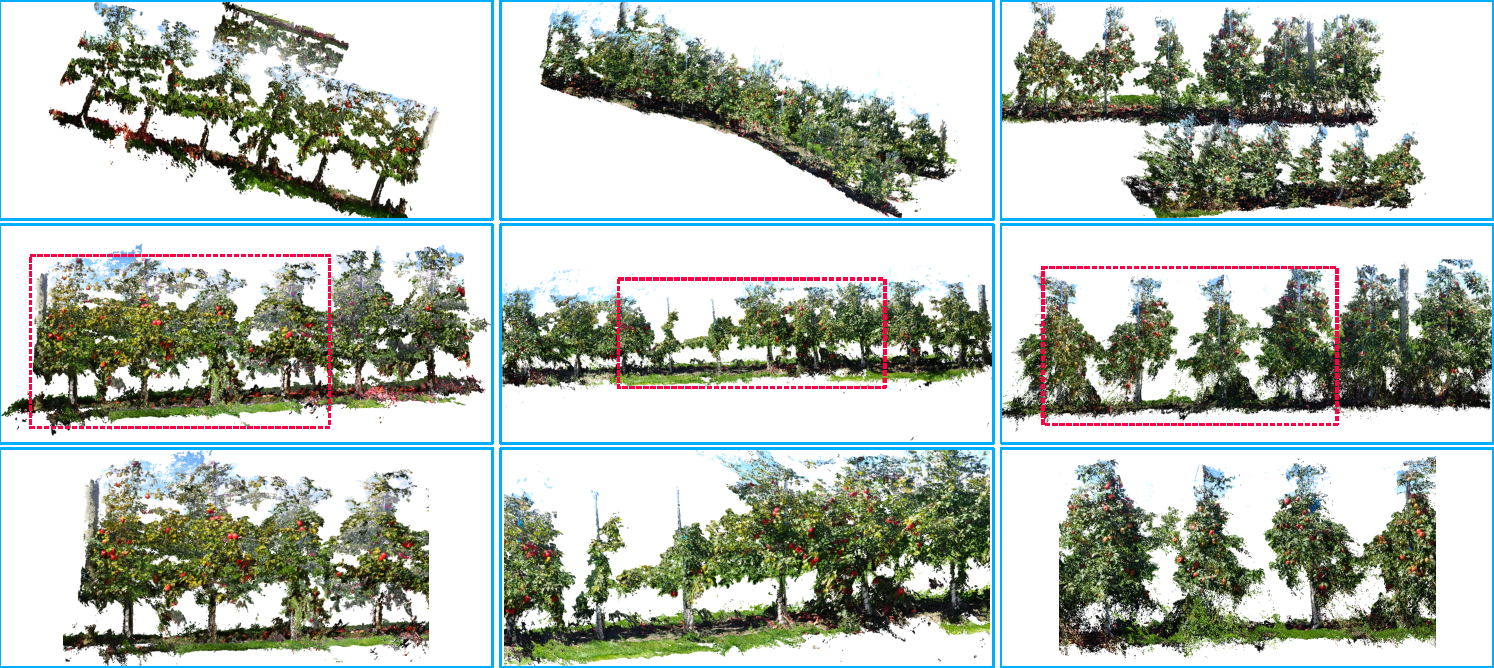
\includegraphics[width =0.99\textwidth]{figures/merge_both/experiment_merge_RGB.pdf}
    \caption[Merged 3D reconstructions for RGB datasets.]{Merged 3D reconstructions from two sides of tree rows for Dataset-1, Dataset-2 and Dataset-3. Rows 1: Input front-side and back-side 3D reconstructions. Rows 2: Output merged 3D models from both sides. Row 3: 3D models are well merged without misalignments from a zoom-in view.}
    \label{fig:dataset2_recons}
\end{figure}


\begin{figure*}[!hbpt]
    \centering
    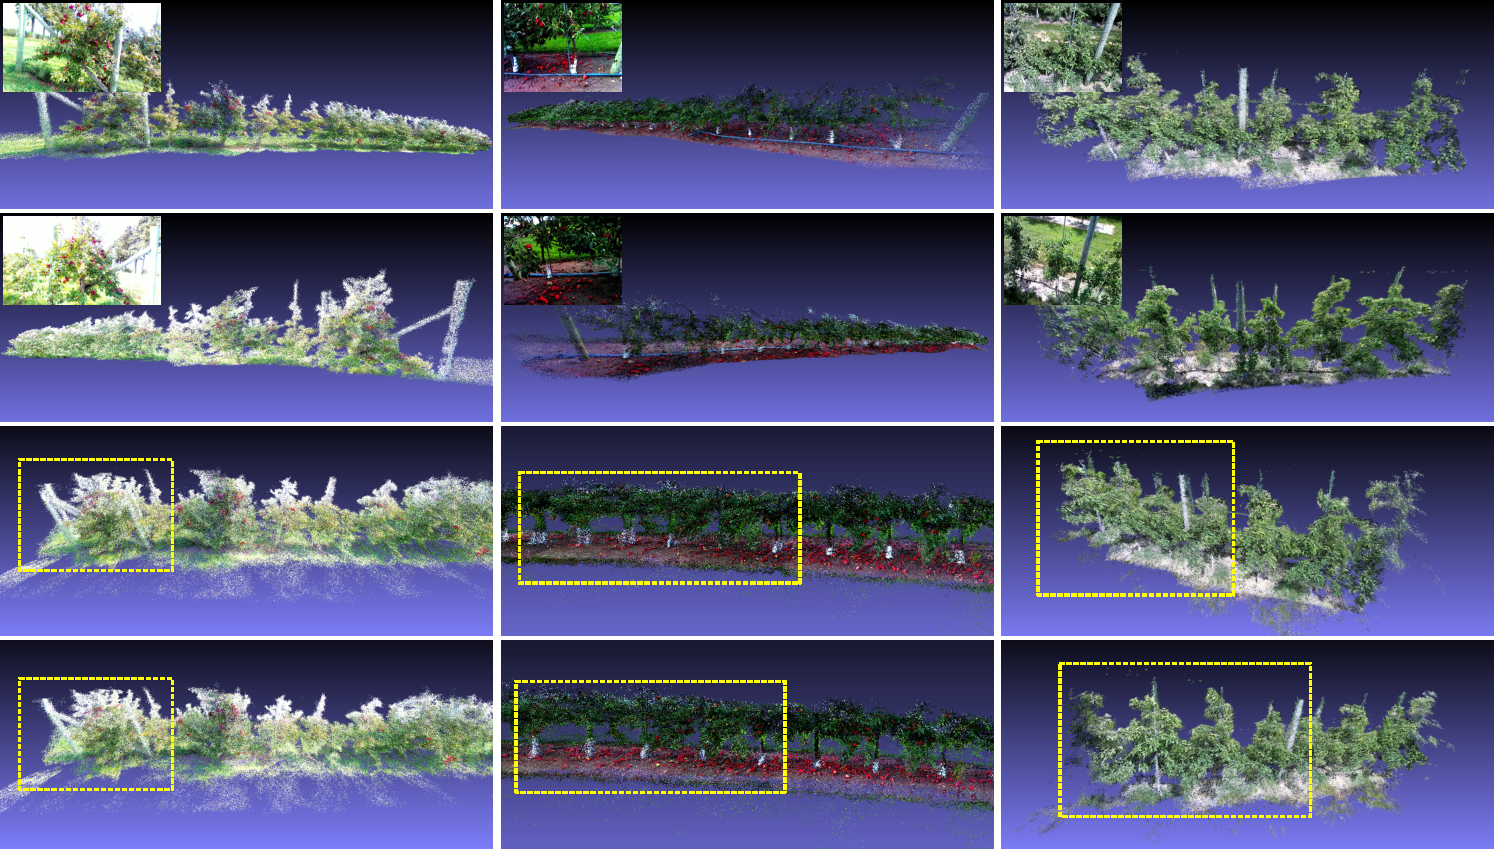
\includegraphics[width=0.99\textwidth]{figures/merge_both/experiment_merge.pdf}
    \caption[Merged 3D reconstructions for RGB-D datasets.]{Merged 3D reconstructions from two sides of tree rows for Dataset-4, Dataset-5 and Dataset-6. Rows 1 and 2: Front-side and back-side 3D reconstructions with scene images. Row 3: Misalignments (yellow boxes) of some landmarks after initial transformation. Row 4: Good 3D models are obtained by eliminating misalignments from semantic BA.}
    \label{fig:Canopy_Test}
    %\vspace*{-2mm}
\end{figure*}



\section{Experimental Insights and Conclusion}

In this chapter, we developed a method for merging reconstructions from two sides of a tree row by exploiting global features (i.e., occlusion boundaries from orthographic views) and semantic information (i.e., detected trunks and local grounds). Our method produces coherent geometric reconstructions solely from camera footage and can be used on a variety of platforms including Unmanned Aerial Vehicles~\cite{techreportroy} and Unmanned Ground Vehicles~\cite{peng2016semantic} which have been demonstrated to navigate through modern orchard environments.

The key idea behind the alignment of orthographic projection boundaries is that 3D reconstructions from two sides vary considerably in terms of geometry (i.e., they are different in scale, and might have different missing parts in the models). This is precisely the reason for applying the Coherent Point Drift (CPD)~\cite{myronenko2010point} method to align them. This iterative method enables us to treat the small changes in geometry as noise/outliers and to achieve approximately correct alignments. The alignment can fail if the input reconstructions from two sides are not accurate enough or have no mutual information. For example, we aim to merge 3D reconstructions of a row of $10$ trees. The 3D model from the front side only reconstructs four trees, whereas the reconstruction from the backside builds the six trees that are not covered (or less than two trees are covered) from the front side. In this case, the alignment of orthographic projection boundaries will fail.


In chapter~\ref{chapter:merge_both}, we show how the merged models highly improve the accuracy of yield estimation by eliminating fruit visible from both sides. Besides, canopy volume can be readily computed from the model based on the segmentation of each tree, and trunk diameter and tree height can be estimated using robust detection and fitting algorithms~\cite{dong2018semantic}. 